\chapter{Back-Propagation}\label{backprop}

One of the most common algorithms used for deep feedforward neural network learning is the \VUname{Back-propagation} algorithm (\cite{rumelhart_learning_1986}), sometimes called \VUname{backprop}. This term is often misunderstood as meaning the whole learning algorithm, whereas in fact this name refers only to the algorithm used for computing the gradient of the network, which is then used by the actual learning algorithm, such as gradient descent (\cite{cauchy_methode_1847}), stochastic gradient descent or more advanced algorithms such as ADAM (\cite{kingma_adam:_2014}).

While Back-propagation is commonly used for computing the gradient of a feedforward neural network, it is not limited to his task. Given a function \( f \left( \VUvec{x}, \VUvec{y} \right) \), the Back-propagation algorithm can be used to compute the gradient of such a function with respect to \( \VUvec{x} \), i. e. \( \nabla_{\VUvec{x}} f \left( \VUvec{x}, \VUvec{y} \right) \). To use the Back-propagation algorithm, it is useful to describe the function with a \VUname{computational graph}. A computational graph is a connected directed acyclic graph with nodes representing variables and edges representing operations, that is functions describing how to compute said variables. For example the equation \( y = f \left( x \right) \) is represented by two nodes, \( x \) and \( y \), and a directed edge from \( x \) to \( y \). The node representing \( y \) is labeled \( f \). This label is applied to the end node as the operation can in general have multiple input variables. Some of these labels may be omitted if the itermediary values are not of interest.

\section{Chain Rule of Calculus}
\begin{theorem}\label{chain_rule}
	Let \( x \) be a real number, \( f : \VUfield{R} \to \VUfield{R} \), \( g : \VUfield{R} \to \VUfield{R} \). Let \( y = f \left( x \right) \) and \( z = g \left( y \right) \). Then
	\[ \frac{\mathrm{d} z}{\mathrm{d} x} = \frac{\mathrm{d} z}{\mathrm{d} y} \frac{\mathrm{d} y}{\mathrm{d} x} \]
\end{theorem}

This theorem can be generalized for vectors:

\begin{theorem}\label{chain_rule_vector}
	Let \( \VUvec{x} \in \VUfield{R}^n \), \( f : \VUfield{R}^n \to \VUfield{R}^m \), \( g : \VUfield{R}^m \to \VUfield{R} \). Let \( \VUvec{y} = f \left( \VUvec{x} \right) \) and \( z = g \left( \VUvec{y} \right) \). Then
	\[ \frac{\partial z}{\partial x_i} = \sum_{j = 1}^{m} \frac{\partial z}{\partial y_j} \frac{\partial y_j}{\partial x_i} \]
	or, in vector notation
	\[ \nabla_{\VUvec{x}} z = \left( \frac{\partial \VUvec{y}}{\partial \VUvec{x}} \right)^T \nabla_{\VUvec{y}} z \]
	where \( \frac{\partial \VUvec{y}}{\partial \VUvec{x}} \) is the Jacobian matrix of \( f \).
\end{theorem}

And this theorem can in turn be similarly generalized for tensors:

\begin{theorem}\label{chain_rule_tensor}
	Let \( \VUmat{X} \) be a tensor, \( f \) and \( g \) functions. Let \( \VUmat{Y} = f \left( \VUmat{X} \right) \) and \( z = g \left( \VUmat{Y} \right) \). Then
	\[ \nabla_{\VUmat{X}} z = \sum_j \left( \nabla_{\VUmat{X}} Y_j \right) \frac{\partial z}{\partial Y_j} \]
	where \( j \) is a tuple of indices for \( \VUmat{Y} \).
\end{theorem}

\section{Applying the chain rule}

In a computational graph, if there exists a directed edge from \( x \) to \( y \), the influence changing \( x \) has on \( y \) is represented by \( \frac{\partial y}{\partial x} \). To compute such influence between two variables which are not directly connected by an edge the chain rule can be used. This is trivial if there is only a singular directed path between the variables. However, consider the following problem:

\begin{figure}[h]
	\centering
	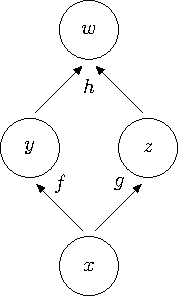
\includegraphics[width=150pt]{images/diamond/diamond.pdf}
	\caption{Diamond-style computational graph}\label{diamond}
\end{figure}

\begin{example}
	Let \( x \), \( y \), \( z \) and \( w \) be real numbers such that \( y = f \left( x \right) \), \( z = g \left( x \right) \) and \( w = h \left( y, z \right) \). The computational graph for this set of variables and operations is in figure \ref{diamond}. The derivative \( \frac{\partial w}{\partial x} \) cannot be computed directly by applying theorem \ref{chain_rule}. Instead a sum over both directed paths must be used:
	\[ \frac{\partial w}{\partial x} = \frac{\partial w}{\partial y} \frac{\partial y}{\partial x} + \frac{\partial w}{\partial z} \frac{\partial z}{\partial x} \]
	This is the result of theorem \ref{chain_rule_vector} where 
	\[ h : \VUfield R^2 \to \VUfield R : 
	\begin{pmatrix}
		y \\
		z
	\end{pmatrix} \mapsto w \]

Generally, in order to find the derivative \( \frac{\partial y}{\partial x} \) the sum of chains of partial derivatives over all directed paths from \( x \) to \( y \) must be taken. This approach becomes computationally infeasible as the number of combinations of all edges increases very quickly with the length of the path. Back-propagation tries to overcome this explosive growth of the number of summands by performing factorization. Therefore, even when an edge is a part of several paths, its gradient is only computed once. This approach reduces computational complexity at the cost of higher memory requirements, a trade-off which may or may not be beneficial depending on the type of problem. For deep feedforward neural networks, the computational graphs are usually complicated and heavily interconnected, which makes such a trade-off a necessity.

The back-propagation algorithm is used to compute a gradient of a given single output variable \( y \) with respect to a set of given input variables \( x^{(i)} \), that is \( \frac{\partial y}{\partial x^{(i)}} \text{ for } i \in \left\{ 1, \dots, n \right\} \). The algorithm can be seen as successively assigning to each node \( u \) of the computational graph the gradient \( \frac{\partial y }{\partial u} \). There are two simplifications to be made for the computational graph:

\begin{remark}\label{backprop-no-dead-ends}
	It can be assumed without loss of generality that from all nodes \( u \) of a given computation graph, there exists a directed path from \( u \) to the output node \( y \). If it were not so, then the gradient for such a node would be \( \frac{\partial y}{\partial u} = 0 \)
\end{remark}
\begin{remark}
	The computational graph can without loss of generality be assumed to only contain such nodes \( u \) that
	\[ \left( \exists i \in \left\{ 1, \dots, n \right\} \right) \left( \exists \text{ a directed path from } x^{(i)} \text{ to } u \right) \]
	This assumption only serves as an optimisation as the excluded nodes do not affect the result of the algorithm and thus can be omitted.
\end{remark}

As a result of the fact that the computational graph is acyclic, all the nodes \( u_1, \dots, u_k \) can be ordered in such a way that if there exists an edge from \( u_j \) to \( u_i \), then \( i < j \) (Reverse topological ordering). Moreover as a result of remark \ref{backprop-no-dead-ends} and the fact that the graph is connected, there holds \( y = u_1 \) and so \( \frac{\partial y}{\partial u_1} = 1 \).

Then, for each node \( u_i \) of the computational graph, its gradient can be written as
\[ \frac{\partial y}{\partial u_i} = \sum_{u_j \in \mathrm{Desc} \left( u_i \right)} \frac{\partial y}{\partial u_j} \frac{\partial u_j}{\partial u_i} \]
where
\[ \mathrm{Desc} \left( u_i \right) = \left\{ u \middle| \exists \text{ a directed edge from } u_i \text{ to } u \right\} \]
If the nodes are reverse topologically ordered and the gradients computed in this order, then each of the necessary partial derivatives needed to compute \( \frac{\partial y}{\partial u_i} \) has already been computed. Using this approach, the gradient for each node is computed only once during the run of the algorithm. \todo{Algorithm - as algorithm 6.5 in Deep learning}

\section{Application of back-propagation to deep feedforward neural networks}\label{backprop_application}

A deep feedforward neural network (also known as a \VUname{multilayer perceptron}) can be seen as a special case of a computational graph. The \( i \)-th layer of such a network can be represented as:
\[ \VUvec h^{(i)} = f^{(i)} \left( \VUvec{h}^{(i - 1)} ; \VUvec{\theta}^{(i)} \right) = \sigma^{(i)} \left( {\VUmat{W}^{(i)}}^T \VUvec h^{(i - 1)} + \VUvec{b}^{(i)} \right) \]
where \( \VUvec{h}^{(i - 1)} \) is the input of the layer, \( \VUvec{h}^{(i)} \) its output and
\[ \VUvec{\theta}^{(i)} = \left( {\VUmat{W}^{(i)}}^T \middle| \VUvec{b}^{(i)} \right)^T \]
are the parameters of the layer (the weights \( \VUmat{W}^{(i)} \) and the bias \( \VUvec{b}^{(i)} \)).

In such a notation, a neural network with input \( \VUvec{x} \) can be represented as
\[ \widehat{\VUvec{y}} = f^{(n)} \circ f^{(n - 1)} \circ \dots \circ f^{(1)} \left( \VUvec{x} \right) \]
where for each layer \( f^{(i)} \) there exist corresponding parameters \( \VUvec{\theta}^{(i)} \). If \( L \) denotes the loss function of the network and \( \VUvec{y} \) is the desired output of the network for the input \( \VUvec{x} \), then the back-propagation algorithm is used to minimize the loss \( J = L \left( \widehat{\VUvec{y}}, \VUvec{y} \right) \).

For simplicity, in the following text the input and predicted output are also denoted as
\[ \VUvec{h}^{(0)} = \VUvec{x} \qquad \text{and} \qquad \VUvec{h}^{(n)} = \widehat{\VUvec{y}} \]

First, the derivative of the loss with respect to the predicted output is taken:
\[ \nabla_{\widehat{\VUvec{y} }} J = \nabla_{\widehat{\VUvec{y}}} L \left( \widehat{\VUvec{y}}, \VUvec{y} \right) \]
Then, for the \( i \)-th layer, theorem \ref{chain_rule_tensor} is used for the activation function \( \sigma^{(i)} \):
\[ \nabla_{\VUvec{a}^{(i)}} J = \nabla_{\VUvec{h}^{(i)}} J \odot {\sigma^{(i)}}' \left( \VUvec{a}^{(i)} \right) \]
where 
\[ \VUvec{a}^{(i)} = {\VUmat{W}^{(i)}}^T \VUvec h^{(i - 1)} + \VUvec{b}^{(i)} \]
From this value, the gradient with respect to the parameters of the layer can be computed as
\[ \nabla_{\VUmat{W}^{(i)}} J = \nabla_{\VUvec{a}^{(i)}} J {\VUvec{h}^{(i - 1)}}^T \]
\[ \nabla_{\VUvec{b}^{(i)}} J = \nabla_{\VUvec{a}^{(i)}} J \]
And for computing the gradients of the layer below:
\[ \nabla_{\VUvec{h}^{(i - 1)}} J = {\VUmat{W}^{(i)}}^T \nabla_{\VUvec{a}^{(i)}} J \]
If the gradients are computed backwards to the order of layers, this ordering is a reverse topological ordering of the computational graph and thus all the values required in each step of the algorithm have already been computed.

This chapter has been sourced from \cite{goodfellow_deep_2016} and \cite{olah_calculus_2015}.
\end{example}
